% =============================================================================
% User guide and algorithm explanation for tree_clustering.py
% Compile with: pdflatex tree_clustering_guide.tex  (twice for TOC/refs)
% =============================================================================
\documentclass[11pt,a4paper]{article}

\usepackage[margin=2.5cm]{geometry}
\usepackage{amsmath,amssymb}
\usepackage{booktabs}
\usepackage{tabularx}
\usepackage{longtable}
\usepackage{enumitem}
\usepackage{graphicx}
\usepackage[dvipsnames,svgnames]{xcolor}
\usepackage{hyperref}
\usepackage{listings}
\usepackage{microtype}
\usepackage{caption}
\usepackage{fancyhdr}
\usepackage{adjustbox}
\usepackage{tikz}
\usetikzlibrary{arrows.meta,positioning,calc,shapes.geometric}

\hypersetup{
  colorlinks=true,
  linkcolor=blue!50!black,
  urlcolor=blue!60!black,
  citecolor=blue!50!black
}

% Cluster palette (matches tree_clustering.py COLOR_PALETTE)
\definecolor{pal00}{HTML}{FF00FF}
\definecolor{pal01}{HTML}{3B82F6}
\definecolor{pal02}{HTML}{10B981}
\definecolor{pal03}{HTML}{F59E0B}
\definecolor{pal04}{HTML}{8B5CF6}
\definecolor{pal05}{HTML}{06B6D4}
\definecolor{pal06}{HTML}{84CC16}
\definecolor{pal07}{HTML}{F97316}
\definecolor{pal08}{HTML}{6366F1}
\definecolor{pal09}{HTML}{14B8A6}
\definecolor{pal10}{HTML}{64748B}
\definecolor{pal11}{HTML}{FBBF24}
\definecolor{pal12}{HTML}{A855F7}
\definecolor{pal13}{HTML}{22C55E}
\definecolor{palNoise}{HTML}{9CA3AF}

\newcommand{\hexswatch}[2]{%
  \textcolor{#1}{\rule{0.9em}{0.9em}}\,%
  \textcolor{#1}{\textbf{\upshape\# #2}}%
}

\lstset{
  basicstyle=\ttfamily\small,
  breaklines=true,
  frame=single,
  columns=fullflexible,
  keepspaces=true,
  showstringspaces=false,
  backgroundcolor=\color{gray!8}
}

\pagestyle{fancy}
\fancyhf{}
\fancyhead[L]{\textit{tree\_clustering.py} user guide}
\fancyhead[R]{\thepage}
\renewcommand{\headrulewidth}{0.4pt}

\title{%
  \textbf{tree\_clustering.py}\\[0.4em]
  \large User Guide and Algorithm Explanation
}
\author{Cursor (Composer)\\[0.25em]
\large under instruction from Hugh Murrell}
\date{\today}

\begin{document}
\maketitle

\begin{abstract}
\texttt{tree\_clustering.py} is a command-line batch tool that implements a
k-DPI clustering workflow.
For each Newick phylogeny in an input directory it parses days-post-infection
(DPI) from the filename, groups tip names, selects a founder tip from the
smallest group id, reroots and ladderizes the tree, runs automatic k-DPI
bipartition clustering, and writes an annotated linear SVG tree plot.
With \texttt{--as-is}, founder selection, reroot, and ladderize are skipped so
clustering uses the loaded topology unchanged.
Optionally it annotates a matching FASTA alignment.
After processing a directory it writes a housekeeping CSV and a pie-chart SVG
summarising cluster-count distributions across CAP samples.
This document is the complete user guide and a detailed description of the
algorithms implemented in the script.
\end{abstract}

\tableofcontents
\newpage

% -----------------------------------------------------------------------------
\section{Introduction}
% -----------------------------------------------------------------------------

\subsection{Purpose}
The script batch-processes phylogenetic trees with a fixed pipeline:
\begin{enumerate}[nosep]
  \item load a phylogenetic tree;
  \item group sequences by a name field;
  \item reroot on a founder;
  \item ladderize;
  \item run k-DPI Auto clustering;
  \item export a DPI-aware tree SVG (and optionally annotate FASTA).
\end{enumerate}
It is intended for batch analysis of many participant trees (typically CAP
cohort Newick files) with consistent parameters.

\subsection{Conventions}
Notable defaults and design choices:
\begin{itemize}[nosep]
  \item default grouping uses delimiter \texttt{\_} and field~3;
  \item k-DPI bipartition objective
        $\min\max(\mathrm{depth}_1,\mathrm{depth}_2)$
        with both children required to meet minimum cluster size;
  \item DPI from mean pairwise tree-path distance;
  \item cluster / noise naming \texttt{\_cl-}$x$ / \texttt{\_cl-n};
  \item linear SVG export with AUTO or legacy DPI branch scaling.
\end{itemize}
Founder selection uses the \emph{tree-path medoid} of the group with the
smallest group id.

\subsection{Requirements}
\begin{itemize}[nosep]
  \item Python~3.9+ (uses \texttt{from \_\_future\_\_ import annotations});
  \item standard library only (no Biopython or other third-party packages).
\end{itemize}

% -----------------------------------------------------------------------------
\section{Command-line usage}
% -----------------------------------------------------------------------------

\subsection{Synopsis}
\begin{lstlisting}
python3 tree_clustering.py INPUT_DIR OUTPUT_DIR [options]
\end{lstlisting}

\subsection{Positional arguments}
\begin{description}[style=nextline,leftmargin=2.2cm,labelwidth=2cm]
  \item[\texttt{INPUT\_DIR}]
    Directory containing Newick tree files.
    Recognised extensions:
    \texttt{.nwk}, \texttt{.newick}, \texttt{.tree}, \texttt{.tre},
    \texttt{.treefile}, \texttt{.txt}.
  \item[\texttt{OUTPUT\_DIR}]
    Directory for SVG trees, optional annotated FASTA,
    \texttt{housekeeping.csv}, and \texttt{housekeeping.svg}.
    Created if missing.
\end{description}

\subsection{Optional arguments}
\begin{longtable}{@{}p{3.6cm}p{2.4cm}p{8cm}@{}}
\toprule
\textbf{Option} & \textbf{Default} & \textbf{Meaning} \\
\midrule
\endfirsthead
\toprule
\textbf{Option} & \textbf{Default} & \textbf{Meaning} \\
\midrule
\endhead
\texttt{--delimiter} & \texttt{\_} &
  Character splitting tip names into fields for grouping. \\
\texttt{--field} & $3$ &
  1-based field index used as the group label. \\
\texttt{--dsr} & $6.5\times10^{-5}$ &
  Daily substitution rate (mutations / site / day);
  see Section~\ref{sec:dsr}. \\
\texttt{--min-size} & $1$ &
  Minimum allowed size of each child after a bipartition.
  Singletons are still reclassified as noise at assignment. \\
\texttt{--max-splits} & $63$ &
  Maximum number of Auto splits (upper bound on $k-1$). \\
\texttt{--scale} & \texttt{auto} &
  SVG branch scale: \texttt{auto} (fit tree + target marks) or
  \texttt{dpi} (legacy: expected depth at $520/16$~px). \\
\texttt{--fasta-dir} & (none) &
  Directory of FASTA files with the same basename as each tree.
  When set, tip names and FASTA headers are annotated with cluster suffixes. \\
\texttt{--no-long-branch-noise} & off &
  Disable removal of tips whose incoming branch exceeds
  $\mathrm{etd}$ (expected pairwise tip distance;
  $\mathrm{etd}=2\times\mathrm{dsr}\times\mathrm{DPI}$). \\
\texttt{--as-is} & off &
  Skip founder selection, reroot, and ladderize; cluster and draw the input
  tree topology as loaded (no \texttt{[Founder]} highlight). \\
\bottomrule
\end{longtable}

\subsection{Examples}
\begin{lstlisting}
# Minimal batch run
python3 tree_clustering.py trees_in/ trees_out/

# Default grouping and annotate FASTA
python3 tree_clustering.py trees_in/ trees_out/ \
  --delimiter _ --field 3 \
  --fasta-dir fasta_in/

# Legacy DPI 1/16 scale, no long-branch pre-noise
python3 tree_clustering.py trees_in/ trees_out/ \
  --scale dpi --no-long-branch-noise

# Cluster without founder / reroot / ladderize
python3 tree_clustering.py trees_in/ trees_out/ --as-is
\end{lstlisting}

% -----------------------------------------------------------------------------
\section{Inputs and outputs}
% -----------------------------------------------------------------------------

\subsection{Tree filenames and DPI}
DPI days are parsed from the tree basename with the regular expression
\begin{center}
\verb|dpi[+|-](\d+)|
\end{center}
(case-insensitive). If several matches occur, the \emph{largest} integer is used.
If none are present, DPI defaults to $14$.

Examples:
\begin{itemize}[nosep]
  \item \texttt{C002\_CAP008\_dpi+79.nwk} $\rightarrow$ DPI $=79$;
  \item \texttt{x\_dpi-14\_dpi+100.nwk} $\rightarrow$ DPI $=100$;
  \item \texttt{plain.nwk} $\rightarrow$ DPI $=14$.
\end{itemize}

CAP identifiers for housekeeping are parsed with \verb|(CAP\d+)|
(e.g.\ \texttt{CAP008}).

\subsection{Tip name grouping}
Tip names are split on \texttt{--delimiter}. Field \texttt{--field}
(1-based) becomes the group label. Existing cluster suffixes of the form
\texttt{\_cl-}$x$, \texttt{\_cl-na}, or \texttt{\_cl-n} are stripped before
grouping.

Example (delimiter \texttt{\_}, field~$3$):
\begin{center}
\texttt{C002\_CAP008\_2000\_env\_pb-AGTCGATC} $\rightarrow$ group \texttt{2000}.
\end{center}

\subsection{Per-tree outputs}
For a tree with stem $S$, $G$ groups and $C$ non-noise clusters, the script writes
\begin{center}
\texttt{$S$\_gr-}$G$\texttt{\_cl-}$C$\texttt{.svg}
\end{center}
into \texttt{OUTPUT\_DIR}.

If \texttt{--fasta-dir} is set, a matching FASTA
(\texttt{$S$.fasta} / \texttt{.fa} / \texttt{.fas} / \texttt{.fna}) is required.
An annotated copy is written to \texttt{OUTPUT\_DIR} under the same filename,
with headers ending in \texttt{\_cl-}$x$ or \texttt{\_cl-n} (noise).
Tree tip labels in the SVG are annotated the same way when FASTA annotation
is enabled.

\subsection{Batch housekeeping outputs}
After all trees are processed:
\begin{description}[style=nextline]
  \item[\texttt{housekeeping.csv}]
    Columns \texttt{CAPid}, \texttt{Groups}, \texttt{Clusters};
    one row per successfully processed tree; sorted by numeric CAP id.
  \item[\texttt{housekeeping.svg}]
    Pie chart of CAP samples binned by cluster count:
    $1$, $2$, $3$--$4$, $5$--$8$, $9$--$16$, \ldots\
    (empty bins omitted).
\end{description}

% -----------------------------------------------------------------------------
\section{Pipeline overview}
% -----------------------------------------------------------------------------

For each tree file the script executes the following stages in order.
With \texttt{--as-is}, the founder, reroot, and ladderize stages are omitted
(Sections~\ref{sec:founder}--\ref{sec:ladder}); layout, clustering, annotation,
and SVG export still run on the loaded rooting and tip order.

\begin{enumerate}
  \item \textbf{Parse} Newick into an in-memory tree; set parent pointers.
  \item \textbf{Parse DPI} from the filename (Section~\ref{sec:dpi}).
  \item \textbf{Group} tip names (Section~\ref{sec:group}).
  \item \textbf{Founder}: take the group with the smallest group id; choose the
        tree-path medoid (Section~\ref{sec:founder})
        (\emph{skipped} if \texttt{--as-is}).
  \item \textbf{Reroot} on the founder (Section~\ref{sec:reroot})
        (\emph{skipped} if \texttt{--as-is}).
  \item \textbf{Ladderize} by subtree depth, ascending (Section~\ref{sec:ladder})
        (\emph{skipped} if \texttt{--as-is}).
  \item \textbf{Layout} assign root-to-node depths and tip row indices.
  \item \textbf{k-DPI Auto} clustering (Section~\ref{sec:kdpis}).
  \item \textbf{Assign} cluster IDs; reclassify singletons as noise;
        number non-noise clusters $1..k$ by tip order (Section~\ref{sec:assign}).
  \item \textbf{Optional FASTA / tip annotation} (Section~\ref{sec:fasta}).
  \item \textbf{SVG export} with AUTO or DPI scale and per-cluster bars
        (solid target, dashed mean pairwise; Section~\ref{sec:svg}).
\end{enumerate}
Finally, write housekeeping CSV and pie chart.

\begin{figure}[htbp]
\centering
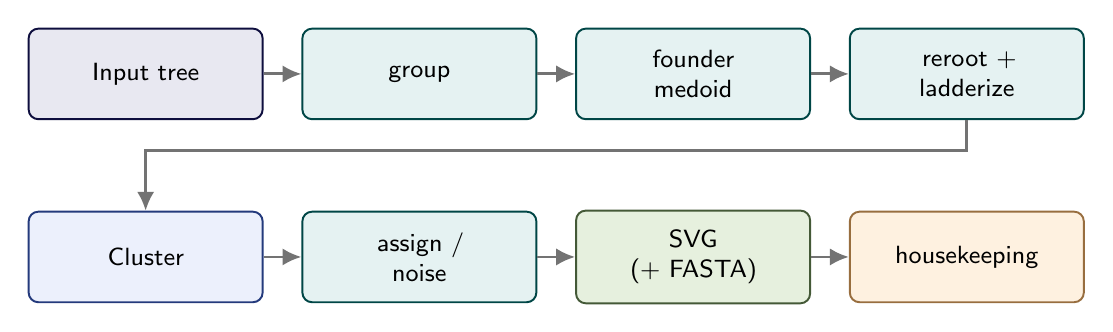
\begin{tikzpicture}[
  font=\sffamily\small,
  node distance=0.55cm and 0.48cm,
  box/.style={
    draw=#1!55!black,
    fill=#1!10,
    rounded corners=3.5pt,
    align=center,
    inner xsep=6pt,
    inner ysep=7pt,
    minimum height=1.15cm,
    text width=2.55cm,
    line width=0.7pt
  },
  box/.default=Teal,
  arr/.style={
    -{Latex[length=2.4mm, width=2.2mm]},
    line width=1.05pt,
    draw=black!55
  }
]
  % Row 1
  \node[box=MidnightBlue] (n1) {Input tree};
  \node[box=Teal, right=of n1] (n2) {group};
  \node[box=Teal, right=of n2] (n3) {founder\\medoid};
  \node[box=Teal, right=of n3] (n4) {reroot +\\ladderize};
  \draw[arr] (n1) -- (n2);
  \draw[arr] (n2) -- (n3);
  \draw[arr] (n3) -- (n4);

  % Row 2
  \node[box=RoyalBlue, below=1.15cm of n1] (n5) {Cluster};
  \node[box=Teal, right=of n5] (n6) {assign /\\noise};
  \node[box=OliveGreen, right=of n6] (n7) {SVG\\(+ FASTA)};
  \node[box=BurntOrange, right=of n7] (n8) {housekeeping};
  \draw[arr] (n5) -- (n6);
  \draw[arr] (n6) -- (n7);
  \draw[arr] (n7) -- (n8);

  % Wrap connector: end of row 1 down/left into start of row 2
  \draw[arr] (n4.south) -- ++(0,-0.38) -| (n5.north);
\end{tikzpicture}
\caption{High-level data flow of \texttt{tree\_clustering.py}
  (default path). With \texttt{--as-is}, the founder medoid and
  reroot\,+\,ladderize stages are skipped.}
\label{fig:pipeline}
\end{figure}

% -----------------------------------------------------------------------------
\section{Tree geometry primitives}
\label{sec:geom}
% -----------------------------------------------------------------------------

Let each edge carry a non-negative length $\ell(u)$ stored as the
\emph{incoming} length of child $u$.
The root-to-node distance $d(u)$ satisfies
\[
  d(\mathrm{root})=0,\qquad
  d(u)=d(\mathrm{parent}(u))+\ell(u).
\]
(The implementation includes $\ell(\mathrm{root})$ in $d(\mathrm{root})$ if
present; Newick roots usually have $\ell=0$.)

\subsection{Path distance}
For tips $a,b$ with lowest common ancestor $\mathrm{lca}(a,b)$,
\[
  \delta(a,b)=d(a)+d(b)-2\,d(\mathrm{lca}(a,b)).
\]

\subsection{Cluster depth (LCA height)}
For a tip set $T$ with $|T|\ge 2$ and $L=\mathrm{lca}(T)$,
\[
  \mathrm{depth}(T)=\max_{t\in T}\bigl(d(t)-d(L)\bigr).
\]
For $|T|<2$, depth is defined as $0$.

\subsection{Mean pairwise distance and DPI}
\[
  \overline{\delta}(T)=\frac{2}{|T|(|T|-1)}\sum_{a<b}\delta(a,b)
  \qquad(|T|\ge 2).
\]
Days-post-infection for a tip set is
\begin{equation}
  \widehat{\mathrm{DPI}}(T)
  =\mathrm{round}\!\left(\frac{\overline{\delta}(T)}{2\,\mathrm{dsr}}\right).
  \label{eq:dpi}
\end{equation}
Equivalent form:
$\mathrm{dpi}=\overline{\delta}/(2\times\mathrm{dsr})$.

\subsection{Expected pairwise tip distance (etd)}
\label{sec:etd}
Under a strict-clock star model, the \emph{expected pairwise tip distance}
(\texttt{etd}) is the expected tree path length between two randomly chosen tips
after $\mathrm{DPI}$ days:
\begin{equation}
  \mathrm{etd}=2\times\mathrm{dsr}\times\mathrm{DPI}.
  \label{eq:etd}
\end{equation}
(The leading factor of~$2$ accounts for mutations accruing independently on both
lineages from their common ancestor.)
Long-branch pre-noise removes tips whose incoming branch exceeds $\mathrm{etd}$.
The SVG / scale-bar \emph{target length} used for vertical marks is the one-sided
quantity
\begin{equation}
  \tau=\mathrm{DPI}\times\mathrm{dsr}
  \label{eq:tau}
\end{equation}
(half of $\mathrm{etd}$), i.e.\ expected root$\to$tip depth for $\mathrm{DPI}$ days.

\subsection{Default daily substitution rate}
\label{sec:dsr}
The default \texttt{dsr} is $6.5\times10^{-5}$ substitutions per site per day.
It is obtained from early-infection parameters assembled by Keele~\emph{et~al.}\
\cite{Keele2008}: reverse-transcriptase error rate
$\mu=2.16\times10^{-5}$ per site per replication, generation time
$t_{\mathrm{gen}}=2$~days, and basic reproductive ratio $R_0=6$, via
\begin{equation}
  \mathrm{dsr}=\frac{\mu\,R_0}{t_{\mathrm{gen}}}
  =\frac{(2.16\times10^{-5})\times 6}{2}
  =6.48\times10^{-5}
  \approx 6.5\times10^{-5}.
  \label{eq:dsr}
\end{equation}
Here $\mu/t_{\mathrm{gen}}$ is the baseline lineage clock (one replication per
generation), and the factor $R_0$ treats Keele's expanding early-infection
regime as raising the \emph{effective} daily substitution rate used when
converting tree path length into days
($\widehat{\mathrm{DPI}}=\overline{\delta}/(2\times\mathrm{dsr})$,
$\mathrm{etd}=2\times\mathrm{dsr}\times\mathrm{DPI}$).
Override with \texttt{--dsr} if a different calibration is preferred.

% -----------------------------------------------------------------------------
\section{DPI from filename}
\label{sec:dpi}
% -----------------------------------------------------------------------------

Let $M$ be the set of integers matched by \texttt{dpi[+|-]$N$} in the
filename. Then
\[
  \mathrm{DPI}=
  \begin{cases}
    \max M & M\neq\emptyset,\\
    14 & \text{otherwise}.
  \end{cases}
\]
This DPI is used as:
\begin{itemize}[nosep]
  \item the Auto split threshold (split only while $\widehat{\mathrm{DPI}}>\mathrm{DPI}$);
  \item the long-branch threshold via~\eqref{eq:etd};
  \item the SVG target length~$\tau$ via~\eqref{eq:tau}.
\end{itemize}

% -----------------------------------------------------------------------------
\section{Grouping}
\label{sec:group}
% -----------------------------------------------------------------------------

For each tip name $s$:
\begin{enumerate}[nosep]
  \item strip a trailing cluster suffix matching
        \texttt{delimiter\,cl-(digits|na|n)};
  \item split on \texttt{delimiter};
  \item if field \texttt{field} exists and is non-empty, use it as the group label.
\end{enumerate}
Group IDs are contiguous integers $0,1,\ldots$ ordered by sorted unique labels.
Tips lacking the field are excluded from grouping (and therefore cannot be
founders).

% -----------------------------------------------------------------------------
\section{Founder selection}
\label{sec:founder}
% -----------------------------------------------------------------------------

Unless \texttt{--as-is} is set, the script chooses a founder tip and then
reroots and ladderizes (Sections~\ref{sec:reroot}--\ref{sec:ladder}).
With \texttt{--as-is}, those steps are skipped and clustering proceeds on the
loaded topology.

Let $G^\star$ be the group with the smallest group id
(group ids are unique, so this choice is unambiguous).
Among tips $T^\star$ of $G^\star$, the founder $f$ is the
\emph{tree-path medoid}
\begin{equation}
  f=\arg\min_{a\in T^\star}\sum_{b\in T^\star}\delta(a,b).
\end{equation}
If $|T^\star|=1$, that tip is the founder.

% -----------------------------------------------------------------------------
\section{Reroot on founder}
\label{sec:reroot}
% -----------------------------------------------------------------------------

Rerooting places the founder as an outgroup child of a new root:
\begin{enumerate}
  \item Walk the path from founder leaf to the old root.
  \item Detach the founder from its parent; let $\ell_{f}$ be the founder edge length.
  \item Invert the remaining spine so the former parent becomes the root of the
        rest of the tree, transferring edge lengths along the flipped path.
  \item Create a new root with children
        $\{$founder, rest$\}$
        and set both edge lengths to $\ell_{f}/2$ (midpoint of the founder edge).
\end{enumerate}
Pairwise tip path distances are preserved under this reroot (undirected metric).

% -----------------------------------------------------------------------------
\section{Ladderize by depth}
\label{sec:ladder}
% -----------------------------------------------------------------------------

For each node $u$, define subtree max depth recursively:
\[
  D(u)=
  \begin{cases}
    \ell(u) & u\text{ leaf},\\
    \ell(u)+\max_{c\in\mathrm{children}(u)} D(c) & \text{otherwise}.
  \end{cases}
\]
Children of every internal node are then sorted by ascending $D(c)$
(``shallow subtrees first'').
Tip display order (top to bottom) follows this child order after layout.

% -----------------------------------------------------------------------------
\section{k-DPI Auto clustering}
\label{sec:kdpis}
% -----------------------------------------------------------------------------

\subsection{Pre-noise (long branches)}
Unless \texttt{--no-long-branch-noise} is set, tips with
$\ell(t)>\mathrm{etd}$ are removed from clustering and later labelled noise.
If all tips would be removed, the filter is abandoned and all tips are kept.

\subsection{Partition tree}
Clustering maintains a binary partition tree of tip sets (``k-DPI leaves'').
Each atomic node stores tip set $T$,
$\widehat{\mathrm{DPI}}(T)$ from~\eqref{eq:dpi}, and $\mathrm{depth}(T)$.

Initially there is one leaf containing all (non-pre-noise) tips.

\subsection{Candidate bipartitions}
To split a tip set $T$ with $|T|\ge 2m$ where $m=\texttt{min-size}$:
\begin{enumerate}
  \item For every phylogeny node, let $R$ be the subset of $T$ descending from it.
  \item If $0<|R|<|T|$, consider the bipartition
        $(L,R)=(T\setminus R,\,R)$.
  \item Accept the candidate only if $|L|\ge m$ and $|R|\ge m$
        (no undersized / noise-only children).
  \item Score $=\max\bigl(\mathrm{depth}(L),\mathrm{depth}(R)\bigr)$.
  \item Choose the bipartition with minimal score.
\end{enumerate}
If no candidate exists, a fallback enumerates nonempty proper unions of
children of $\mathrm{lca}(T)$ (for polytomies with $2$--$20$ children).

\subsection{Which leaf to split (Auto)}
Among atomic leaves with size $\ge 2m$, not marked unsplittable, and with
$\widehat{\mathrm{DPI}}>\mathrm{DPI}_{\mathrm{target}}$,
Auto selects the leaf with largest DPI (ties: larger size).

\subsection{Auto loop}
Repeat until no eligible leaf remains or \texttt{max-splits} is reached:
\begin{enumerate}[nosep]
  \item find leaf to split;
  \item apply best bipartition (or mark unsplittable and continue);
  \item count one successful split.
\end{enumerate}

\begin{figure}[htbp]
\centering
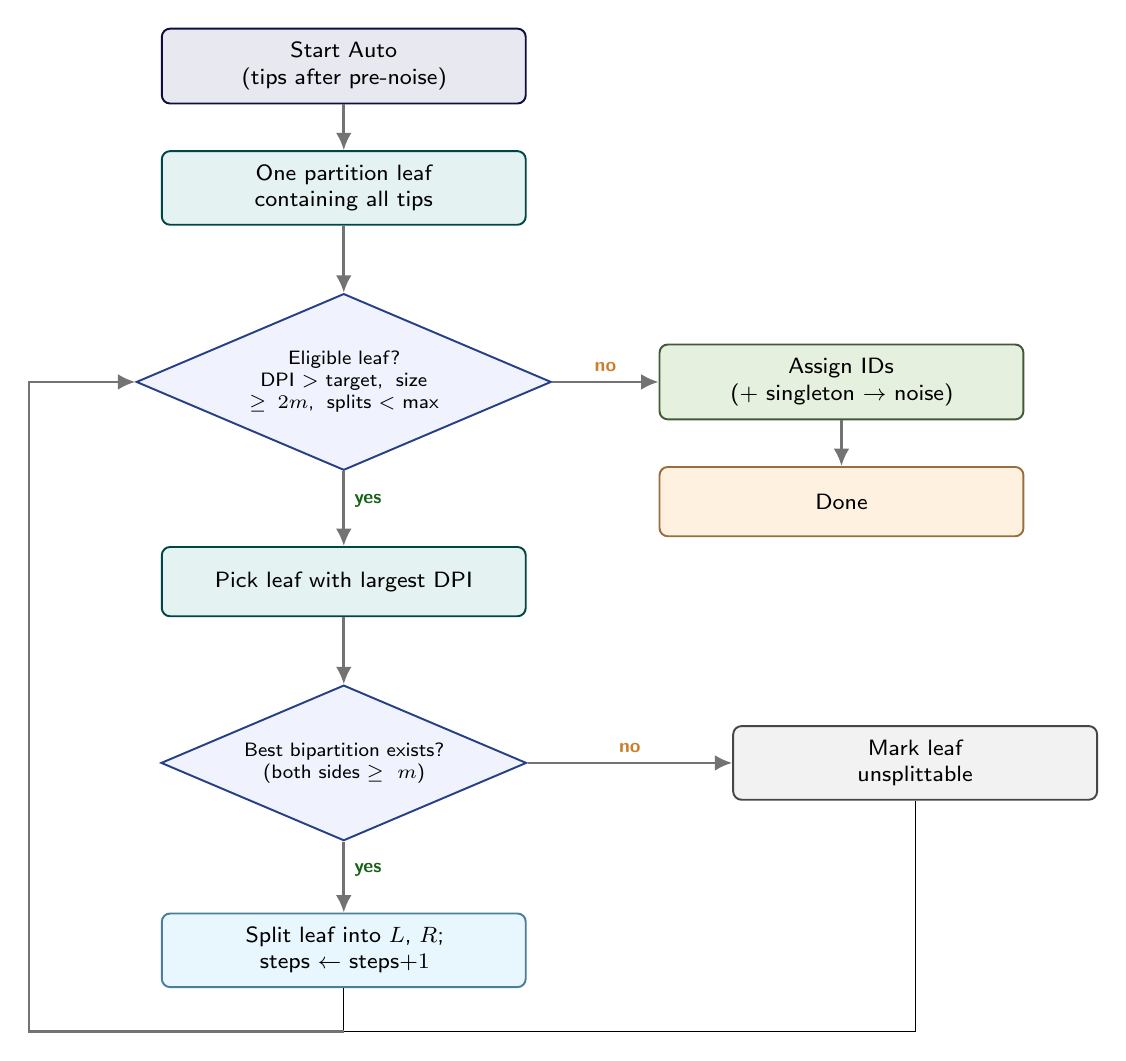
\begin{tikzpicture}[
  font=\sffamily\footnotesize,
  node distance=0.58cm,
  box/.style={
    draw=#1!55!black,
    fill=#1!10,
    rounded corners=3pt,
    align=center,
    inner xsep=6pt,
    inner ysep=5pt,
    text width=4.2cm,
    minimum height=0.88cm,
    line width=0.7pt
  },
  box/.default=Teal,
  decision/.style={
    diamond,
    aspect=2.35,
    draw=RoyalBlue!60!black,
    fill=RoyalBlue!8,
    align=center,
    inner sep=1pt,
    text width=3.2cm,
    font=\sffamily\scriptsize,
    line width=0.7pt
  },
  arr/.style={
    -{Latex[length=2.2mm, width=2mm]},
    line width=0.95pt,
    draw=black!55
  },
  yes/.style={font=\sffamily\scriptsize\bfseries, text=ForestGreen!70!black},
  no/.style={font=\sffamily\scriptsize\bfseries, text=BurntOrange!80!black}
]
  \node[box=MidnightBlue] (start) {Start Auto\\(tips after pre-noise)};
  \node[box=Teal, below=of start] (init) {One partition leaf containing all tips};
  \node[decision, below=0.85cm of init] (eligible) {Eligible leaf?\\DPI $>$ target,\; size $\ge 2m$,\; splits $<$ max};

  % Exit right when finished (keep clear of the unsplittable column)
  \node[box=OliveGreen, right=1.35cm of eligible] (assign) {Assign IDs\\(+ singleton $\to$ noise)};
  \node[box=BurntOrange, below=of assign] (done) {Done};

  % Loop body down the centre
  \node[box=Teal, below=0.95cm of eligible] (pick) {Pick leaf with largest DPI};
  \node[decision, below=0.85cm of pick] (bip) {Best bipartition exists?\\(both sides $\ge m$)};
  \node[box=ProcessBlue, below=0.9cm of bip] (split) {Split leaf into $L$, $R$;\quad steps $\leftarrow$ steps$+1$};
  % Unsplittable to the right of the query; return goes down then left to join
  \node[box=Gray, right=2.6cm of bip] (unspl) {Mark leaf\\unsplittable};

  \draw[arr] (start) -- (init);
  \draw[arr] (init) -- (eligible);
  \draw[arr] (eligible) -- node[no, above] {no} (assign);
  \draw[arr] (assign) -- (done);

  \draw[arr] (eligible) -- node[yes, right, pos=0.4] {yes} (pick);
  \draw[arr] (pick) -- (bip);
  \draw[arr] (bip) -- node[yes, right, pos=0.4] {yes} (split);
  \draw[arr] (bip.east) -- node[no, above] {no} (unspl.west);

  % Meet under Split; unspl goes fully down to that depth, then left to join
  \coordinate (meet) at ([yshift=-0.55cm]split.south);
  \coordinate (railbot) at ([xshift=-1.35cm]eligible.west |- meet);
  \draw (split.south) -- (meet);
  \draw (unspl.south) -- (unspl.south |- meet) -- (meet);
  \draw[arr] (meet) -- (railbot) -- (railbot |- eligible.west) -- (eligible.west);
\end{tikzpicture}
\caption{AUTO k-DPI clustering loop.
  An eligible partition leaf has DPI above the filename target, size at least
  $2m$ ($m=\texttt{min-size}$), and is not marked unsplittable.
  Each successful bipartition increments the split counter; the loop also stops
  when \texttt{max-splits} is reached.
  After the loop, Section~\ref{sec:assign} assigns cluster IDs and reclassifies
  singletons as noise.}
\label{fig:kdpi-auto}
\end{figure}

% -----------------------------------------------------------------------------
\section{Cluster assignment and noise}
\label{sec:assign}
% -----------------------------------------------------------------------------

After Auto finishes, atomic leaves are classified as follows:
\begin{enumerate}
  \item Leaves with $|T|<m$ become noise.
  \item \textbf{Singleton reclassification:} every remaining leaf with $|T|=1$
        is reclassified as noise \emph{before} ID assignment
        (even when $m=1$).
  \item Remaining non-noise leaves are sorted by the minimum tip-row index of
        their members (top of the ladderized tree first).
  \item They receive contiguous IDs $1,2,\ldots,k$.
  \item Pre-noise tips and all noise leaves map to cluster id $-1$.
\end{enumerate}
Display / FASTA suffixes:
\begin{itemize}[nosep]
  \item noise ($\mathrm{id}=-1$): \texttt{\_cl-n}
  \item cluster $x\ge 1$: \texttt{\_cl-}$x$
\end{itemize}

% -----------------------------------------------------------------------------
\section{Optional FASTA annotation}
\label{sec:fasta}
% -----------------------------------------------------------------------------

When \texttt{--fasta-dir DIR} is supplied:
\begin{enumerate}
  \item Locate \verb|DIR/$S$.{fasta,fa,fas,fna}| for tree stem $S$.
  \item For each FASTA header, strip any old cluster suffix, look up the
        cluster id, and append \texttt{\_cl-}$x$ or \texttt{\_cl-n}.
  \item Write the annotated FASTA to \texttt{OUTPUT\_DIR} (same basename).
  \item Rename tree tip labels correspondingly so the SVG shows annotated names.
\end{enumerate}
If no matching FASTA exists, that tree fails with an error
(other trees continue).

% -----------------------------------------------------------------------------
\section{SVG export}
\label{sec:svg}
% -----------------------------------------------------------------------------

\subsection{Layout}
After clustering, tips are drawn top-to-bottom in ladderized order.
An extra top spacer row holds the scale bar above the first tip.
Horizontal position of a node is
\[
  x=5+d(u)\cdot x_{\mathrm{scale}}.
\]
Branch region width is $W=520$~px.

\subsection{Scale modes}
\paragraph{AUTO (default).}
Fit depth
\[
  D_{\mathrm{fit}}=\max\bigl(D_{\mathrm{tree}},\,\tau,\,
  \max_c\bigl(d(\mathrm{lca}_c)+\tau\bigr),\,
  \max_c\bigl(d(\mathrm{lca}_c)+\overline{\delta}_c/2\bigr)\bigr)
\]
where the last two maxima run over non-noise clusters $c$ (so every cluster
target bar and mean-pairwise bar remains inside the plot). Then
$x_{\mathrm{scale}}=W/D_{\mathrm{fit}}$.
When DPI was detected in the filename, the scale-bar label is
\texttt{($N$ DPI @ dsr)}.

\paragraph{DPI (legacy, \texttt{--scale dpi}).}
Place $\tau$ at $W/16=32.5$~px:
$x_{\mathrm{scale}}=(W/16)/\tau$.

\subsection{Per-cluster bars}
\label{sec:cluster-bars}
For each non-noise cluster $c$ with tip set $T_c$ and
$L_c=\mathrm{lca}(T_c)$, two vertical lines are drawn in the cluster palette
colour of $c$, spanning only the vertical extent of $T_c$'s tip rows
(clamped into the branch region if needed). No text annotation is attached.

\paragraph{Solid target bar.}
At expected one-sided depth $\tau=\mathrm{DPI}\times\mathrm{dsr}$:
\[
  x_c^{\mathrm{target}}=5+\bigl(d(L_c)+\tau\bigr)\,x_{\mathrm{scale}}.
\]
This is the Auto stopping threshold: a cluster with
$\widehat{\mathrm{DPI}}>\mathrm{DPI}$ still needs splitting.

\paragraph{Dashed mean-pairwise bar.}
Let $\overline{\delta}_c$ be the mean pairwise tree-path distance among tips
in $T_c$ (undefined for a singleton, so no dashed bar is drawn).
Place a dashed line (stroke-dasharray $6\,4$) at the equivalent one-sided
depth $\overline{\delta}_c/2$:
\[
  x_c^{\mathrm{mpd}}=5+\bigl(d(L_c)+\overline{\delta}_c/2\bigr)\,x_{\mathrm{scale}}.
\]
Because
$\widehat{\mathrm{DPI}}_c=\mathrm{round}(\overline{\delta}_c/(2\times\mathrm{dsr}))$,
the dashed bar sits at or to the \emph{left} of the solid bar precisely when
the cluster does not need a further split
($\widehat{\mathrm{DPI}}_c\le\mathrm{DPI}$).
A dashed bar to the \emph{right} of the solid bar flags a cluster that still
exceeds the target.

Tip diamonds use half-diagonal $5$~px;
both cluster bars use stroke width~$2$.

\subsection{Colours and legend}
\begin{itemize}[nosep]
  \item Tip diamonds: cluster colour (noise grey \hexswatch{palNoise}{9ca3af}).
  \item Tip labels: group colour (founder highlighted magenta); optional
        \texttt{[Founder]} suffix.
  \item Legend: groups with $(n,\widehat{\mathrm{DPI}})$ and clusters with
        $(n,\widehat{\mathrm{DPI}})$, plus noise count.
\end{itemize}

\subsection{Example plots}
Figures~\ref{fig:ex-cl1} and~\ref{fig:ex-cl4} show real batch outputs produced by
\texttt{tree\_clustering.py} (AUTO scale). Both trees were rerooted on a founder,
ladderized by depth, clustered with k-DPI Auto, and drawn with per-cluster
bars (solid target, dashed mean pairwise) and a group/cluster legend.

\begin{figure}[htbp]
\centering
\adjustbox{max height=0.55\textheight, max width=\textwidth, center}{%
  \includegraphics{images/CAP338_cl1.pdf}%
}
\caption{Single-cluster example
  (\texttt{C002\_CAP338\_2000\_\ldots{}dpi+25\_gr-1\_cl-1.svg};
  $s{=}14$ tips, max depth $\approx 0.00157$).
  Filename DPI is~$25$, with scale bar \texttt{(25 DPI @ 5e-05)}.
  All tips form one non-noise cluster, so diamonds share cluster colour~1.
  A solid vertical target bar in that colour is drawn at
  $\mathrm{lca}+\tau$ (here the founder-rerooted root), spanning only the
  cluster tip rows; a dashed bar at $\mathrm{lca}+\overline{\delta}/2$ shows
  the observed mean pairwise depth.
  When Auto has finished, the dashed bar should sit at or left of the solid bar.
  Tip labels use the group colour palette; the founder tip is marked
  \texttt{[Founder]} in magenta and sits as the outgroup after rerooting.
  The top spacer row holds the scale bar; the right-hand legend lists the single
  group as \texttt{2000 ($n$, DPI)} and cluster~\texttt{1} similarly.
  Noise tips (if any) appear grey and are listed under Noise.}
\label{fig:ex-cl1}
\end{figure}

\begin{figure}[htbp]
\centering
\adjustbox{max height=0.55\textheight, max width=\textwidth, center}{%
  \includegraphics{images/CAP333_cl4.pdf}%
}
\caption{Multi-cluster example
  (\texttt{C002\_CAP333\_2000\_\ldots{}dpi+32\_gr-1\_cl-4.svg};
  $s{=}11$ tips, max depth $\approx 0.0174$).
  Filename DPI is~$32$, with scale bar \texttt{(32 DPI @ 5e-05)}.
  One time-point group is present (\texttt{gr-1}).
  k-DPI Auto produced four non-noise clusters (\texttt{cl-4}) plus two noise tips:
  tip diamonds and cluster bars use palette colours~$1$--$4$;
  noise diamonds are grey.
  Each cluster has a solid target bar at $\mathrm{lca}+\tau$ and a dashed
  mean-pairwise bar at $\mathrm{lca}+\overline{\delta}/2$, covering only
  the vertical span of its tips---so later (deeper) clusters have marks further
  to the right.
  Finished clusters have the dashed bar at or left of the solid bar.
  Tip name colours track the group; the founder is highlighted in magenta with
  \texttt{[Founder]}.
  Tip suffixes \texttt{\_cl-}$x$ / \texttt{\_cl-n} match optional FASTA annotation.}
\label{fig:ex-cl4}
\end{figure}

% -----------------------------------------------------------------------------
\section{Housekeeping pie chart}
\label{sec:pie}
% -----------------------------------------------------------------------------

Each CAP sample contributes its non-noise cluster count $C$ to a bin:
\begin{center}
\begin{tabular}{cc}
\toprule
$C$ & Bin label \\
\midrule
$\le 1$ & \texttt{1} \\
$2$ & \texttt{2} \\
$3$--$4$ & \texttt{3-4} \\
$5$--$8$ & \texttt{5-8} \\
$9$--$16$ & \texttt{9-16} \\
$\vdots$ & powers-of-two intervals \\
\bottomrule
\end{tabular}
\end{center}
Only non-empty bins appear as pie slices, ordered by lower endpoint.

% -----------------------------------------------------------------------------
\section{Default parameters (summary)}
% -----------------------------------------------------------------------------

\begin{center}
\begin{tabular}{@{}ll@{}}
\toprule
Parameter & Default \\
\midrule
Daily substitution rate (\texttt{dsr}) & $6.5\times10^{-5}$ \\
DPI if absent from filename & $14$ \\
Group delimiter / field & \texttt{\_} / $3$ \\
Min cluster size & $1$ \\
Max Auto splits & $63$ \\
SVG scale mode & \texttt{auto} \\
Branch plot width & $520$~px \\
Long-branch pre-noise & enabled \\
\bottomrule
\end{tabular}
\end{center}

% -----------------------------------------------------------------------------
\section{Failure modes and exit codes}
% -----------------------------------------------------------------------------

\begin{itemize}
  \item Per-tree failures (parse error, missing group field, missing FASTA when
        required, etc.) are reported on stderr; other trees continue.
  \item Exit code $0$: all trees succeeded.
  \item Exit code $1$: bad arguments / empty input directory.
  \item Exit code $2$: at least one tree failed.
\end{itemize}

% -----------------------------------------------------------------------------
\section{Worked numerical sketch}
% -----------------------------------------------------------------------------

Suppose $\mathrm{dsr}=6.5\times10^{-5}$ and filename DPI $=14$. Then
\[
  \tau=14\times6.5\times10^{-5}=9.1\times10^{-4},\qquad
  \mathrm{etd}=1.82\times10^{-3}.
\]
A tip set with mean pairwise path distance
$\overline{\delta}=2.1\times10^{-3}$ has
\[
  \widehat{\mathrm{DPI}}
  =\mathrm{round}\!\left(\frac{2.1\times10^{-3}}{2\times6.5\times10^{-5}}\right)
  =\mathrm{round}(16.15)=16>14,
\]
so Auto will attempt to split it (subject to size and bipartition constraints).
After a successful split into children with DPI $\le 14$, Auto stops on those
leaves.

% -----------------------------------------------------------------------------
\section{File map}
% -----------------------------------------------------------------------------

\begin{center}
\begin{tabular}{@{}ll@{}}
\toprule
Path & Role \\
\midrule
\texttt{tree\_clustering.py} & Implementation (this guide) \\
\texttt{latex/tree\_clustering\_guide.tex} & This document \\
\texttt{latex/images/} & Example SVG/PDF figures \\
\texttt{latex/Makefile} & Build PDF via \texttt{pdflatex} \\
\bottomrule
\end{tabular}
\end{center}

% -----------------------------------------------------------------------------
\section{Versioning note}
% -----------------------------------------------------------------------------

If script and document disagree, treat \texttt{tree\_clustering.py} as
authoritative and update this guide accordingly.

\appendix
\section{Colour palette (clusters)}
Cluster id $c\ge 0$ uses palette entry $c\bmod 14$.
Hex codes below are printed in the corresponding colour, with a swatch:
\begin{center}
\small
\begin{tabular}{@{}c l@{}}
\toprule
Index & Hex \\
\midrule
0  & \hexswatch{pal00}{ff00ff} \\
1  & \hexswatch{pal01}{3b82f6} \\
2  & \hexswatch{pal02}{10b981} \\
3  & \hexswatch{pal03}{f59e0b} \\
4  & \hexswatch{pal04}{8b5cf6} \\
5  & \hexswatch{pal05}{06b6d4} \\
6  & \hexswatch{pal06}{84cc16} \\
7  & \hexswatch{pal07}{f97316} \\
8  & \hexswatch{pal08}{6366f1} \\
9  & \hexswatch{pal09}{14b8a6} \\
10 & \hexswatch{pal10}{64748b} \\
11 & \hexswatch{pal11}{fbbf24} \\
12 & \hexswatch{pal12}{a855f7} \\
13 & \hexswatch{pal13}{22c55e} \\
\bottomrule
\end{tabular}
\end{center}
Group colours start at palette index~$1$ (group $g$ $\rightarrow$ index
$(g+1)\bmod 14$). Noise uses \hexswatch{palNoise}{9ca3af}.

\begin{thebibliography}{1}

\bibitem{Keele2008}
Brandon~F. Keele, Elena~E. Giorgi, Jesus~F. Salazar-Gonzalez, Julie~M. Decker,
Kimmy~T. Pham, Maria~G. Salazar, Chuanxi Sun, et~al.
\newblock Identification and characterization of transmitted and early founder
virus envelopes in primary {HIV}-1 infection.
\newblock {\em Proceedings of the National Academy of Sciences of the United
States of America}, 105(21):7552--7557, 2008.
\newblock doi:\href{https://doi.org/10.1073/pnas.0802203105}{10.1073/pnas.0802203105}.

\end{thebibliography}

\end{document}
